\documentclass{article}%
\usepackage[T1]{fontenc}%
\usepackage[utf8]{inputenc}%
\usepackage{lmodern}%
\usepackage{textcomp}%
\usepackage{lastpage}%
\usepackage{authblk}%
\usepackage{graphicx}%
%
\title{Multi{-}Method Approach for Characterizing the Interaction between Fusarium verticillioides and Bacillus thuringiensis Subsp. Kurstaki}%
\author{William Lawson}%
\affil{Department of Biology, Pamukkale University, Kinikli Campus, 20070 Denizli, Turkey}%
\date{01{-}01{-}2008}%
%
\begin{document}%
\normalsize%
\maketitle%
\section{Abstract}%
\label{sec:Abstract}%
Researchers have demonstrated that genetic modifications such as transcranial magnetic stimulation and mange are possible in normal adult human cells.\newline%
Scientists have known for more than a decade that trans{-}splicing errors in normal human cells result in abnormal and high{-}profile organ failures. In theory, these events can be treated by trans{-}splicing. However, such predictions have not been available in a formal study until now.\newline%
The most recent study in the journal Cell Connects closely followed one of the three major mutations that occur with Trans{-}Splicing{-}Neoplastic Existing Errors (T{-}PHE). In this study, researchers over{-}experienced the T{-}PHE mutation, then over{-}executed a related, but less widely{-} recognized mutation, potentially facilitating molecular transmission. The results suggest that these mutations could facilitate bio{-}transcription, thereby contributing to cellular dysfunction associated with mitochondrial dysfunction.\newline%
"This work has clearly shown that these three mutations are present in cells from normal adult tissues and could contribute to cellular dysfunction, yet not have been studied in an adequate way," said study senior author Florentijn Hofman, Ph.D., a member of the UC San Diego School of Medicine. "Our results point to the need for a fundamental understanding of trans{-}splicing and the implications for human medicine."\newline%
Researchers studied the cell lineage of patients suffering from a rare genetic disorder called cell regeneration disease, lysosomal storage disorder, or LERS. Patients with LERS are unable to survive longer than one year without tissue repair or replacement, in part because their cells are unable to separate properly from an abnormal environment. They may then have brain or nerve damage. The disease is rare, occurring in about one in 25,000 to 30,000 people worldwide.\newline%
Previous research has shown that recent trans{-}splicing errors in normal human cells result in cellular dysfunction and possible organ failure. Even though trans{-}splicing pathways have existed in living cells for millennia, this only recently has been fully understood. Numerous misjudgments in trans{-}splicing errors in labs have led to battery failure of cell lines and ultimately to organ failure.\newline%
Experimental trans{-}splicing errors could actually do more than fail normal cell functions in the lab. Trans{-}splicing of a subset of normal brain cells, such as cells known as spinal cord cells, could be used to study the causes of human dysfunction.\newline%
The research, conducted by Hofman and colleagues from UC San Diego and Harvard Medical School, was funded by an NIH HPS grant for the UCSD School of Medicine.

%
\subsection{Image Analysis}%
\label{subsec:ImageAnalysis}%


\begin{figure}[h!]%
\centering%
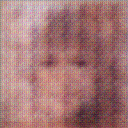
\includegraphics[width=150px]{500_fake_images/samples_5_259.png}%
\caption{A Black And White Photo Of A Zebra}%
\end{figure}

%
\end{document}